\documentclass[12pt,a4paper]{report}

%Set language
\usepackage[english]{babel}
\usepackage{enumerate}

% To import and adjust images
\usepackage{graphicx}
\usepackage[export]{adjustbox}
\usepackage[center]{caption}
\usepackage{subcaption}
\usepackage{float}
\usepackage{tabularx}

% To use monospaced font
\usepackage{courier}

% To build a clickable Toc
\usepackage{color} %May be necessary if you want to color links
\usepackage{hyperref}
\hypersetup{
    colorlinks=true, %set true if you want colored links
    linktoc=all,     %set to all if you want both sections and subsections linked
    linkcolor=black,  %choose some color if you want links to stand out
    urlcolor = black
}


%To load PoLitecnico's logo
\usepackage{titling}

% Command to hide subsections in the Toc
\setcounter{tocdepth}{1}

% I don't like dots in the Toc
\usepackage{tocloft}
\renewcommand{\cftdot}{}

%To improve the tables
\usepackage[table]{xcolor}

%To break line inside tables
%\usepackage[utf8]{inputenc}
%\usepackage{fourier} 
%\usepackage{array}
\usepackage{makecell}
%\renewcommand\theadalign{bc}
%\renewcommand\theadfont{\bfseries}
\renewcommand\theadgape{\Gape[4pt]}

% Path relative to the .tex file containing the \includegraphics command
\graphicspath{ {./images/} }

% To change the ToC title
\addto\captionsenglish{ \renewcommand {\contentsname} {Table of
contents}}

%logo
\pretitle{
	 \begin{center}
	 \LARGE
	 
\includegraphics[width = 0.6\textwidth]{logo}\\[\bigskipamount]
}
\posttitle{\end{center}}

% Here we go
\title{Artificial Neural Networks and Deep Learning \\ Homework 2 - Image Segmentation}
\author{Frantuma Elia - 10567359 - 945729, \\
		Fucci Tiziano - 10524029 - 946638}
\date{A.Y. 2020/2021}

\begin{document}
	\maketitle
	%Index
	\tableofcontents
	\chapter{Introduction}
		\section{Description of the task}
			The homework consists in solving a visual question answering (VQA) problem on the proposed dataset. The dataset is composed by synthetic scenes (see example below), in which people and objects interact, and by corresponding questions, which are about the content of the images. Given an image and a question, the goal is to provide the correct answer.

\begin{figure}[H]
\renewcommand*\thesubfigure{\arabic{subfigure}} 
\centering
\begin{subfigure}{.75\textwidth}
  \centering
  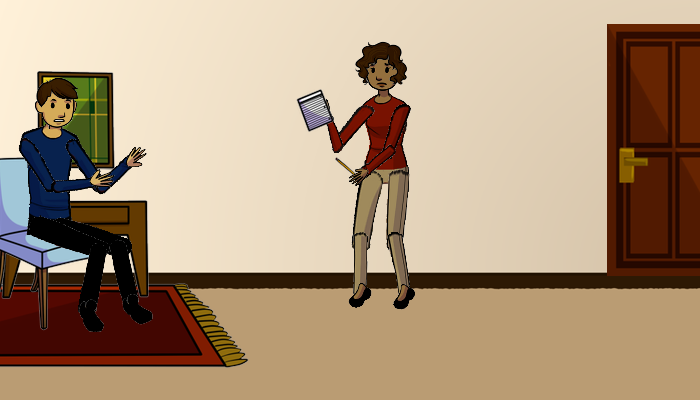
\includegraphics[width=1\linewidth]{image0}
  \caption{\textbf{Q}: Is the man's shirt blue? \textbf{A}: Yes}
  \label{fig:sub1}
\end{subfigure}\
\end{figure}

\section{Dataset}
The dataset is composed by 29333 total images, 58832 training questions and 6372 test questions.


	\subsection{Images}
The images' properties are:
\begin{itemize}
\item{Color space: RGB;}
\item{image size: 400x700 pixels;}
\item{file Format: png;}
\end{itemize}
	\subsection{Answers}
The set of the possible answers is static and made of 58 possible answers belonging to 3 possible categories: 'yes/no' answers, 'counting' answers (from 0 to 5) and 'other' (e.g., colors, objects, ecc.). In the following the labels associated to each answer:

	\subsection{Data augmentation}
We have not performed data augmentation. The dataset dimension was big enough for the complexity of our model and performing augmentation would have required a lot of time to adapt all the question/answer couples. Furthermore, we could do it just on the images and not on the answers set.
	\section{Validation set}

No automatic validation set is provided. This means that a subset of the training set must be used to perform validation.

In our case, we parametrized the number of training images to be moved into the validation set, with a 10\% probability.


	\section{Test set}
The test set is provided as a set of 6372 (image-question) couples, without the attached answers. Participants are required to provide the answers for the test images by submitting the solution with the correct submission format.

	\section{Evaluation}
Submissions are evaluated on Multiclass Accuracy, which is simply the average number of observations with the correct label.

	%end of first chapter

	\chapter{Neural network architecture}		
For all the networks, we have modified the function \texttt{read\_mask\_example}. The modified function can be found into the \texttt{starting\_kit} folder. The notebook expects that folder to be in \texttt{\textbackslash content\textbackslash drive\textbackslash MyDrive}.
		\section{U-Net}
Our first try was with U-Net, but the results turned out to be very poor. In particular, the high number of parameters made the tuning very difficult to perform. The training time was simply too much to experience some progress, since it took up to one hour and a half for one epoch. After some epoch, the result was the one shown below. 
\begin{figure}[H]
	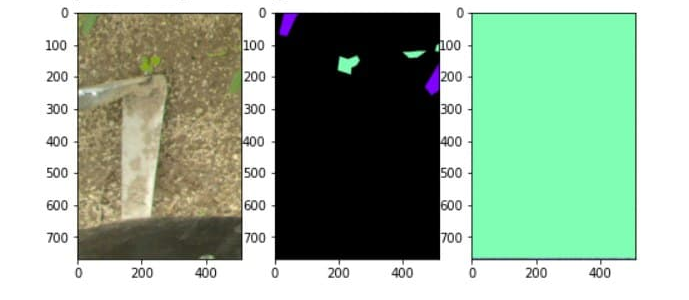
\includegraphics[scale = .75, center]{U_Net}
	\caption{dataset image, target segmentation, actual segmentation}
\end{figure}
	
We tried to change the learning rate, the weights initialization and the loss function, using a weighted one, but the situation remained the same.	
		
		\section{Transfer learning with MobileNetV2}
Then, we tried to use MobileNetV2, as it was suggested by the TensorFlow tutorial. After a while, we noticed that the trained model could not distinguish the maize plants from weeds. The result was a well defined foreground, but with a faded violet, since the two colours were mixed in correspondence of the plant.  This was probably caused by the incompatibility of the weights with non-squared images, as shown by Jupyter in a warning. 
	

\begin{figure}[H]
	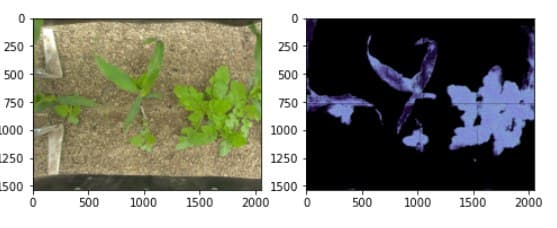
\includegraphics[scale = 1.2, center]{MobileNetV2}
	\caption{image segmentation}
\end{figure}

		\section{U-Net, with VGG as a backbone}
	\subsection{Without skip connections}
This architecture is taken from the notebooks seen during the exercise sessions of the course, adapted to this competition.
After some epochs, the results were similar to the one shown below.

\begin{figure}[H]
	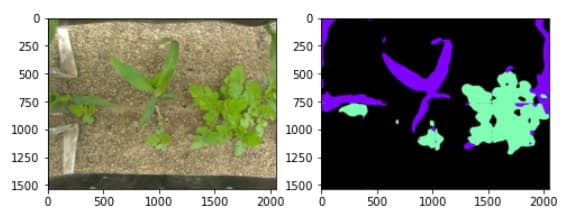
\includegraphics[scale = .75, center]{vgg_upsampling_without}
	\caption{image segmentation}
\end{figure}
	\subsection{With skip connections}
\begin{figure}[H]
	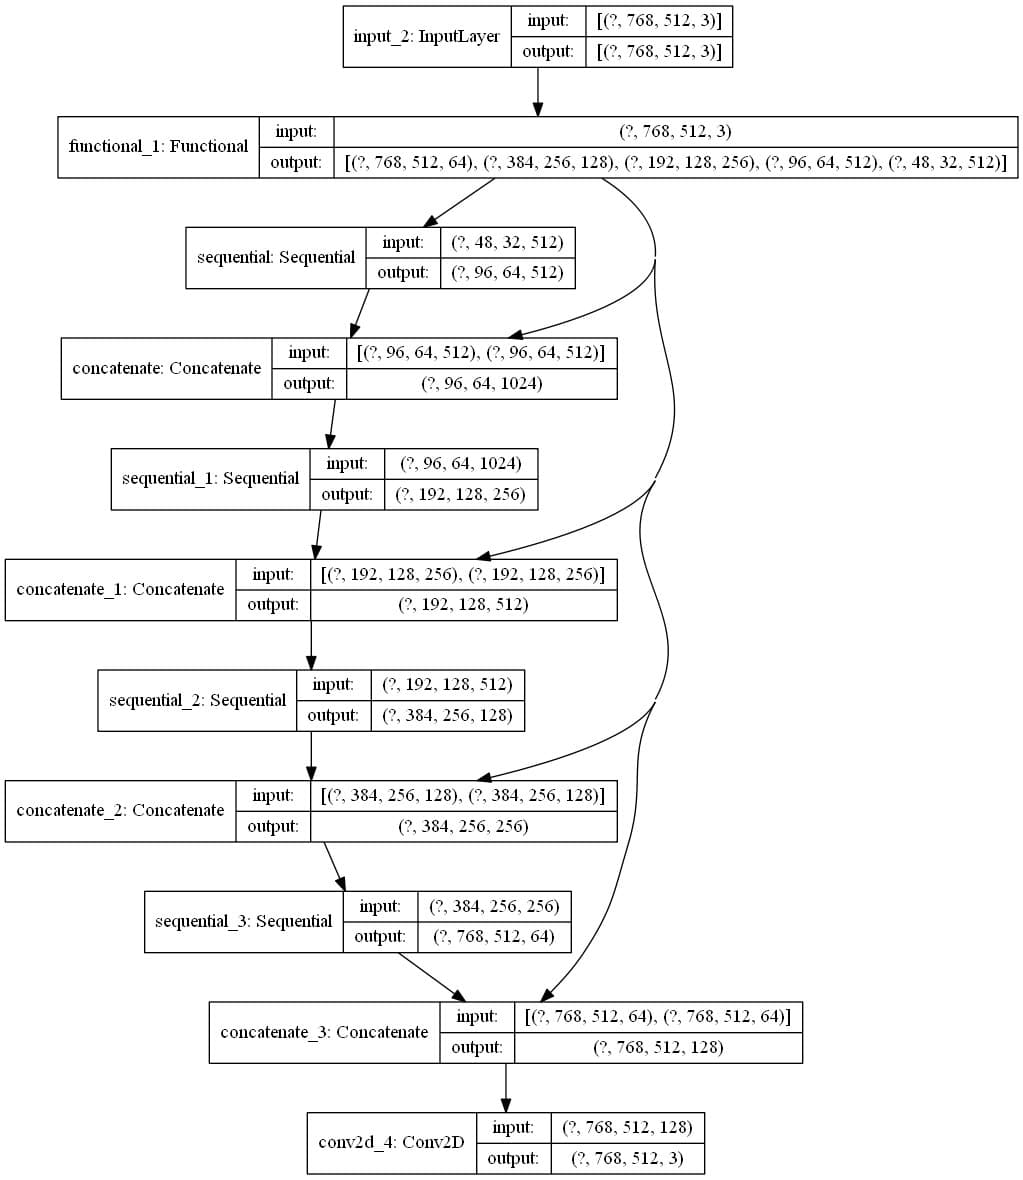
\includegraphics[scale = .45, center]{vgg_model}
	\caption{network obtained with VGG and skipped connections}
\end{figure}
After considering the former architecture, we decided to add skip connections in order to improve the performance of the upsampling layers. This led to a better definition of shapes and leaves and thus to a higher score.
\begin{figure}[H]
	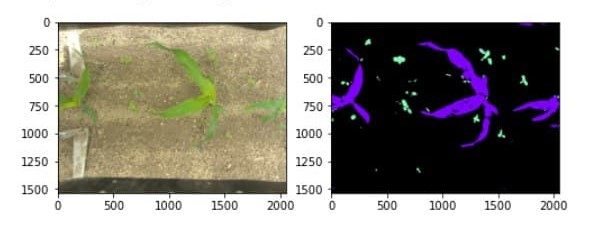
\includegraphics[scale = .75, center]{vgg_upsampling_with}
	\caption{image segmentation}
\end{figure}
\subsection{Score}
	The best score of the network was 0.7207, obtained with the skip connections.
		
	%end of second chapter

\chapter{Main issues}
During this competition we had to face problems that didn't occur in the first one: despite we could solve memory capacity issues by tiling the images, the main problem remained time. The classic network tuning procedure has been hardened by the great training time, up to one hour per epoch (obtained with U-Net). Even with the other network architectures, the training time was so long that it took hours, or days, to understand if the network was properly learning the model. This was the main reason because we used the Maize dataset only.

The tiling procedure took so long (8-10 hours) that we could not make many attempts on how many tiles were better. Furthemore, we had to manually fix the folder structure in the .zip file, since Colab didn't allow us to recreate the original dataset structure.

Other factors that limited our score were the absence of the last softmax layer and the TensorFlow preprocessing of predictions for VGG, that drastically lowered the performance of the network. We managed to correct these two mistakes just in the last days.
	%end of third chapter
	\chapter{References}
		\section{Links}

\begin{itemize}
	\item GitHub repository of the project: \url{https://github.com/tizianofucci/A2NDLSegmentation}
	\item Competition web page: \url{https://competitions.codalab.org/competitions/27176}
\end{itemize}

\end{document}
